\chapter{Methodology} \label{chap:methodology}

In this chapter, we outline the methodology employed to develop and assess the
performance of \ChristBERT{}. Sec.~\ref{sec:corpus} provides an overview of the
various data sources utilized in constructing the pre-training corpus, as well
as the procedures implemented for extracting text from each source. We also
detail the pre-training and initial language modeling evaluation process in
Sec.~\ref{sec:pre-training} and Sec.~\ref{sec:lm_eval}, respectively. Finally,
the downstream tasks on which we evaluate model performance are introduced in
Sec.~\ref{sec:fine-tuning}. To provide an appropriate comparison, we describe
our choice of performance metrics and introduce the experimental setup including
baseline models. 

\section{Corpus Creation} \label{sec:corpus}

\begin{table}[htb]
    \centering
    \begin{tabular}{lrrrr}
    \toprule
    \bfseries Dataset & \bfseries \# Documents & \bfseries \# Sentences & \bfseries \# Words & \bfseries Size (MB) \\
    \midrule
    Hpsmedia & 277,357 & 16,314,452 & 405,316,578 & 3,117 \\
    Springer Nature & 258,000 & 14,158,151 & 259,284,884 & 1,984 \\
    PubMed Central & 90,273 & 8,644,017 & 220,033,966 & 1,609 \\
    PhD Theses & 7,486 & 4,665,850 & 90,380,880 & 646 \\
    Medical Wikipedia & 75,585 & 3,254,135 & 49,594,111 & 362 \\
    MIMIC-IV Notes & 330,486 & 49,351,295 & 733,952,748 & 5,310 \\
    Web Crawl & 93,642 & 4,024,816 & 68,797,358 & 512 \\
    \midrule
    \bfseries Summary & \bfseries 1,132,829 & \bfseries 100,412,716 & \bfseries 1,827,360,525 & \bfseries 13,540 \\
    \bottomrule
    \end{tabular}
    
    \caption[Overview of datasets contained in the pre-training corpus]{
        Overview of datasets contained in the pre-training corpus. The table
        provides details about each dataset, including the number of documents,
        sentences, words, and their size in megabytes. The final corpus includes
        all listed datasets and amounts to roughly 13.5 GB of pre-training
        data.}
    \label{tab:corpus_stats}
\end{table}

Main shortcomings of existing German medical domain models include the limited
availability of training data due to the sensitive nature of medical information
and strict data privacy regulations. Furthermore, many existing biomedical
Transformer models~\cite{lentzen2022critical, bressem2024medbert} are
pre-trained or evaluated on proprietary datasets, hindering independent model
verification and validation. Previous studies~\cite{martin2020camembert,
dada2023impact, bressem2024medbert} concluded that training data diversity and
quantity are more important than excessive data cleaning, which insignificantly
affected downstream performance. Following these findings, we compiled a 13.5 GB
large and highly varying German biomedical and clinical corpus, focusing on data
quantity over quality. In order to mitigate the aforementioned shortcomings, we
primarily relied on public datasets with only two private data sources included,
to ensure reproducibility and accessibility of the \ChristBERT{} models.
Tab.~\ref{tab:corpus_stats} summarizes the pre-training corpus, including
descriptive statistics about the number of documents, sentences, words, and size
of each incorporated dataset.

\subsection{Data Sources and Text Extraction}

\paragraph{Hpsmedia}
Hpsmedia is a German publisher specializing in medical content primarily
targeted at healthcare professionals. Hpsmedia publishes three healthcare
journals \textit{Pflegewissenschaften (Nursing Sciences)}, \textit{Pädagogik der
Gesundheitsberufe (Pedagogy of Health Professions)} and \textit{Geschichte der
Gesundheitsberufe (History of Health Professions)}, which are available in print
and online. All journals publish articles in German and are peer-reviewed by
experts in the respective fields according to the international reviewing
standard BMJ \cite{smith2006peer}. The articles cover a wide range of topics
within the healthcare domain including aspects of health and nursing care,
pedagogy, didactics, curricula, education in healthcare professions and the
history of healthcare professions. We were kindly provided with the full-text
content of the journals in CSV format by Hpsmedia. The CSV files were processed
using the \textsc{Pandas} \cite{mckinney2010data} Python library to extract the
text content of the articles, which was then included in the pre-training
corpus. The Hpsmedia dataset consists of 277,357 documents totaling to 3,117 MB
of data.

\paragraph{Springer Nature}
Springer Nature is a prominent global publisher of academic content, known for
its extensive collection of high-quality journals, books, and research materials
across various disciplines, including science, technology, and medicine.

For the extraction of text from Springer Nature publications, the Springer
Nature API~\cite{springernature} was utilized. The API offers multiple
endpoints, e.g. metadata, full-text (TDM) as well as a wide range of constraint
parameters to filter for desired publications, which are returned in XML format.
This allowed for a systematic filtering for open-access publications in German.
For our purposes, the open-access API was first queried for metadata of articles
and books related to the subjects of \textit{biomedicine}, \textit{public
health}, \textit{pharmacy}, \textit{dentistry} and \textit{life sciences}. The
returned XML data was then processed to extract abstracts and Digital Object
Identifiers (DOI) of each publication, respectively. Subsequently, the set of
DOIs was used to make bulk API calls to the TDM endpoint to subsequently fetch
the full-text content of the publications. In a final step, the extracted
abstracts and full-text content were both incorporated into the pre-training
corpus accounting for a total of 258,000 documents and 1,984 MB of data.

\paragraph{PubMed Central}
PubMed Central (PMC) is a free digital repository of full-text scientific
literature in the field of biomedicine and life sciences and created as an
extension of PubMed \cite{white2020pubmed}, which holds bibliographic references
and abstracts for essentially all publications in the biomedical sciences. Both
repositories are maintained by the National Center for Biotechnology Information
(NCBI), a part of the United States National Library of Medicine (NLM). The PMC
archive provides access to a collection of over 10 million research articles,
reviews, and other scientific publications from a wide range of biomedical and
life science journals. Not all articles in PMC are available for text mining or
other reuse as many are under copyright. The \textit{PMC Open Access Subset}
\cite{pmcoa} contains those articles made truly freely available to the public
under Creative Commons or similar licenses that allow more liberal
redistribution and repurpose than the majority of licensed and copyrighted
articles from subscription access journals deposited in PMC.

\begin{figure}[!htb]
    \centering
    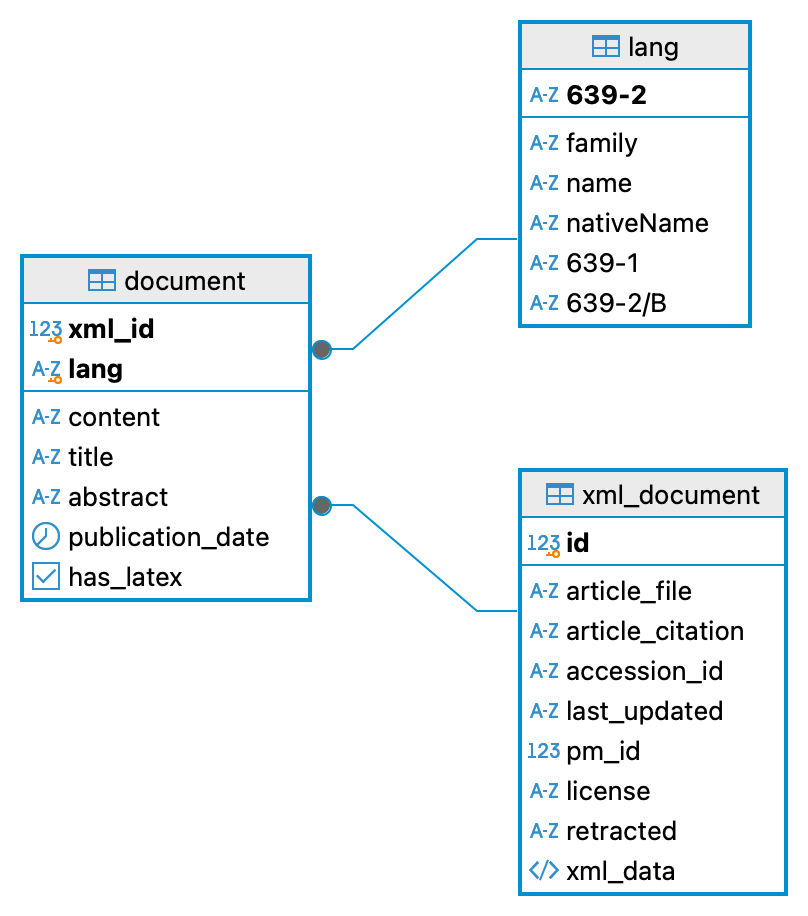
\includegraphics[width=0.5\textwidth]{pmc_erd}
    \caption[Database design for PMC translation]{The diagram shows the database
    relations for translation management. The raw XML files with their metadata
    are stored in the \texttt{xml\_document} table, while the \texttt{document}
    table contains the extracted text data with both PubMed ID and the language
    of a document as its primary keys. Languages are foreign keys to the
    corresponding entity in the \texttt{lang} relation according to the ISO
    639-3 standard.}
    \label{fig:pmc_erd}
  \end{figure}

PMC stores content in XML format, which is structured according to the Journal
Article Tag Suite (JATS) standard, a widely used archival markup format for
journal articles. The JATS XML files are made available by NLM for bulk download
through their PMC FTP Service \cite{pmcoa}. We downloaded the December 2024
baseline package of the PMC Open Access Subset and transferred the XML files
with appropriate metadata such as PubMed ID and publication date to a
\textsc{PostgreSQL} database for further processing. The database design is
shown in Fig.~\ref{fig:pmc_erd}, which is represented by an entity-relationship
diagram. The XML files and their corresponding metadata are stored in the
\texttt{xml\_document} table by leveraging the native support of
\textsc{PostgreSQL} for XML data types. For our needs, we extracted the title,
abstract, full-text content and language of the articles from the XML markup by
utilizing the \textsc{Pubmed Parser} \cite{achakulvisut2020} Python library,
which supports parsing of the JATS XML format. The extracted text data was then
stored in the \texttt{document} table, which contains the PubMed ID and language
of each document as its primary keys. The language of each document is
represented as a foreign key to the \texttt{lang} table, which contains the ISO
639-3 language codes. The \texttt{lang} table is used to ensure data integrity
and consistency across the database.

In order to leverage the large amount of English-language content available in
PMC, we translated the English articles to German using the \textbf{NLLB
200}~\cite{costa2022no} neural machine translation model in its 1.3 billion
distilled variant. Translation was performed on two Nvidia GeForce RTX 3090 24
GB GPUs, while leveraging the \textit{NLLB-API} \cite{nllbAPI} library for
parallel processing. The translation posed a significant computational
challenge, which was addressed by limiting the publications to be translated to
those published in the third and fourth quarters of 2020. This decision was
based on an analysis of article distribution over the past seven years, which is
depicted in Fig.~\ref{fig:histogram}. The analysis revealed a notable peak in
publications in 2022, potentially influenced by the COVID-19 pandemic and the
emergence of generative AI. To ensure that the translated content was not overly
biased towards the COVID-19 pandemic and mitigate the presumably uniform writing
style resulting from generative AI, we selected the year 2020 for our
translations. Likewise, given our computational constraints, we chose the third
and fourth quarters of 2020, as the quarterly distribution of articles in that
year indicated a more feasible volume of publications as seen in
Fig.~\ref{fig:histogram_2020}. Translated documents were saved back to the
database in the \texttt{document} table, but with an updated language key set to
\texttt{de} for German. Further data filtering encompassed the removal of
articles with less than 40 characters and those containing \LaTeX{} markup.
Fig.~\ref{fig:translation} summarizes the described steps for PMC translation as
a flowchart. The translated and natively German articles were then combined into
a single dataset, resulting in a total of 90,272 documents and 1,609 MB of text
data.

\begin{figure}[htbp]
    \centering
    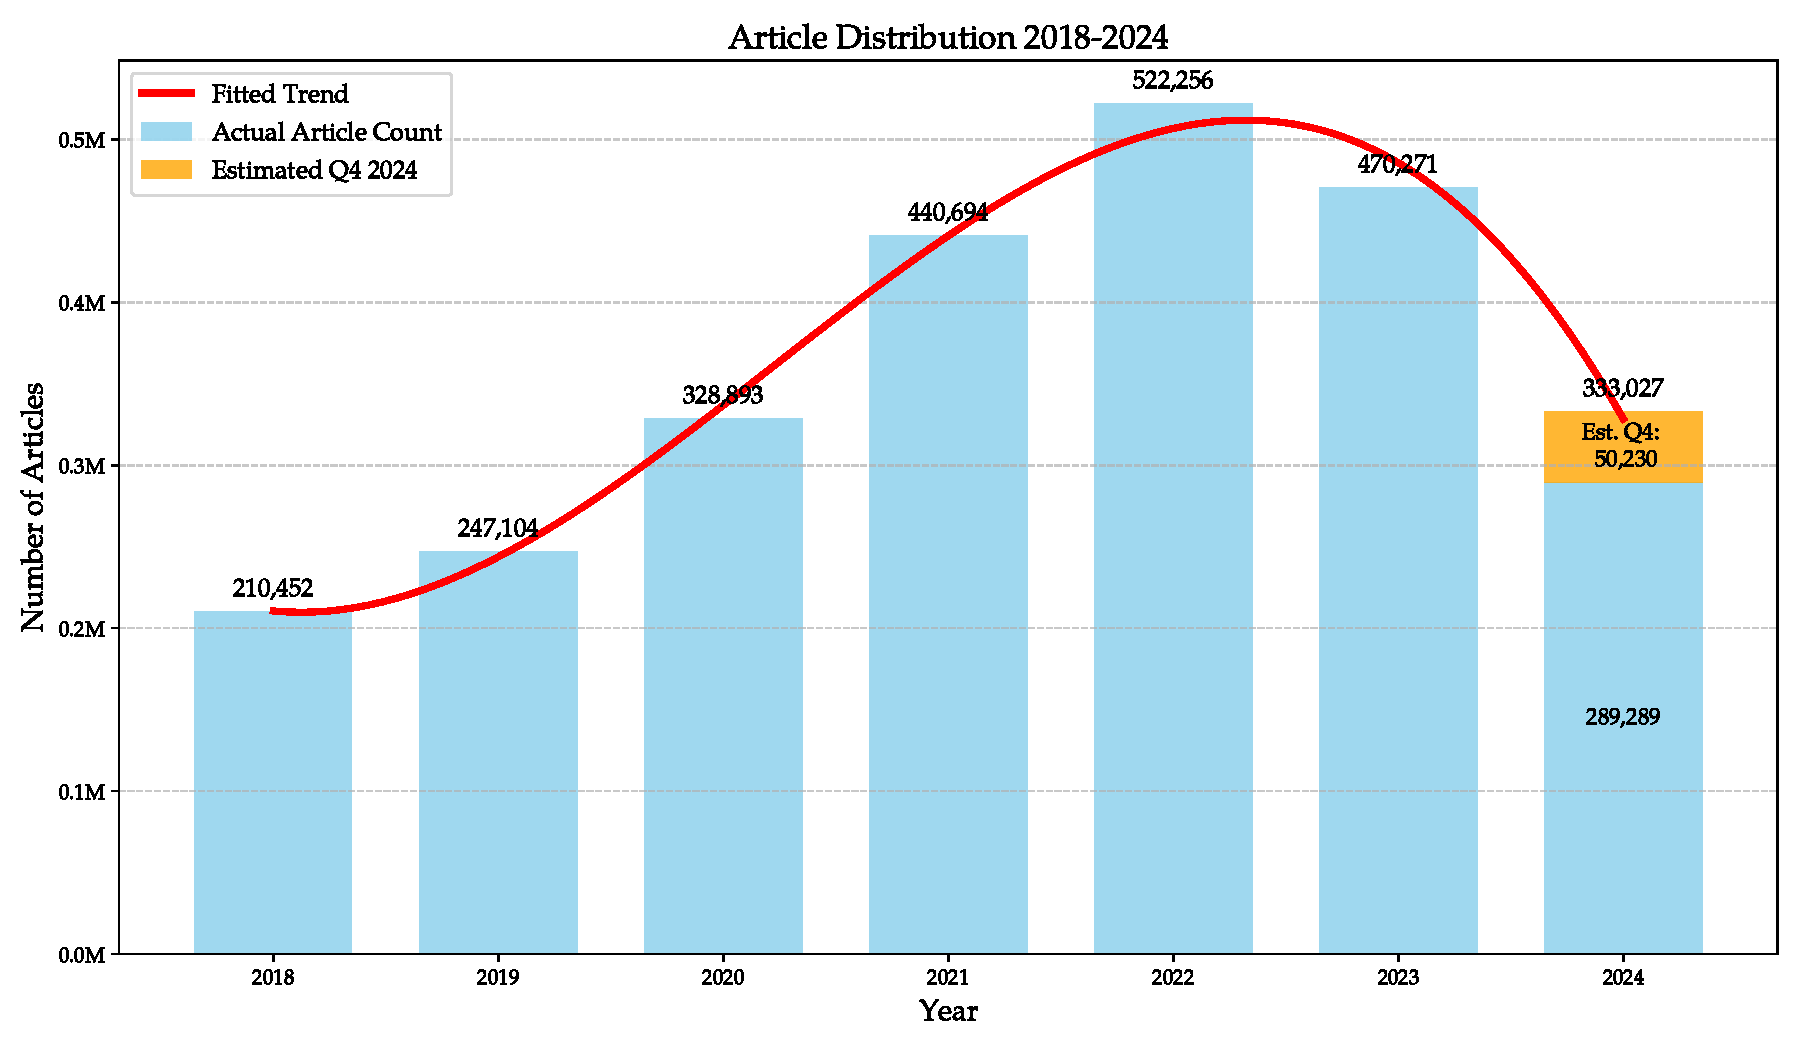
\includegraphics[width=0.9\textwidth]{histogram}
    \caption[Distribution of PMC articles from 2018-2024]{This histogram shows
    the annual number of articles published in PMC from 2018-2024, with a fitted
    trend line indicating the overall growth and decline of article counts. The
    estimated article count for Q4 2024 was approximated based on the maximum
    article count of the past years (50,230).}
    \label{fig:histogram}
\end{figure}
\begin{figure}[htbp]
    \centering
    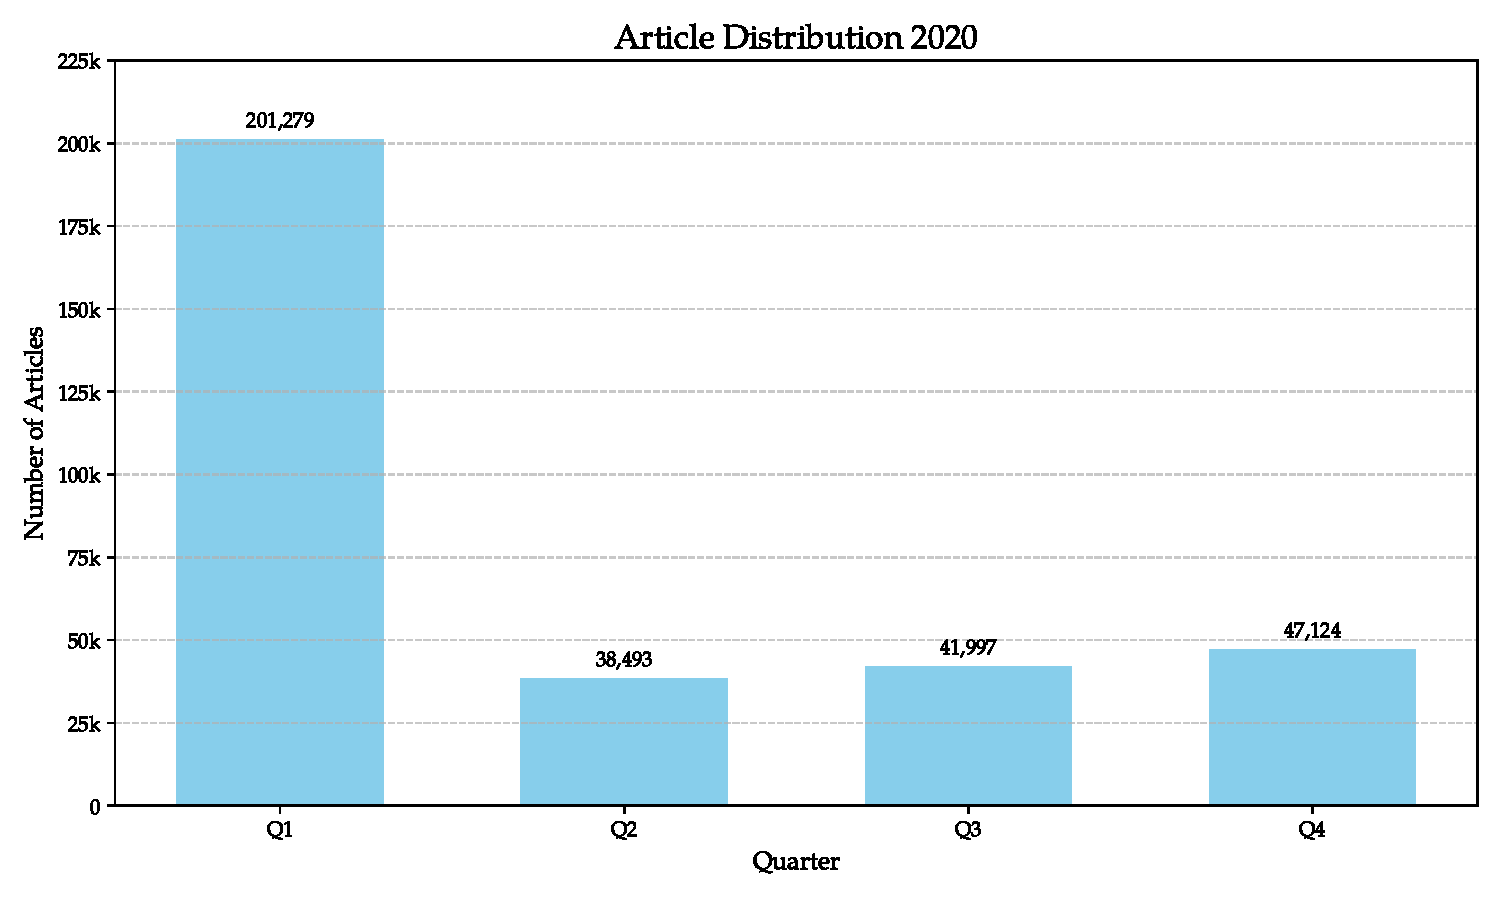
\includegraphics[width=0.9\textwidth]{histogram_2020}
    \caption[Quarterly distribution of PMC articles in 2020]{The histogram
    shows the quarterly number of articles published in PMC in 2020, with a
    peak in Q1 at 201,279 articles, followed by a drop in the subsequent
    quarters.}
    \label{fig:histogram_2020}
\end{figure}

\begin{figure}[p]
    \centering
    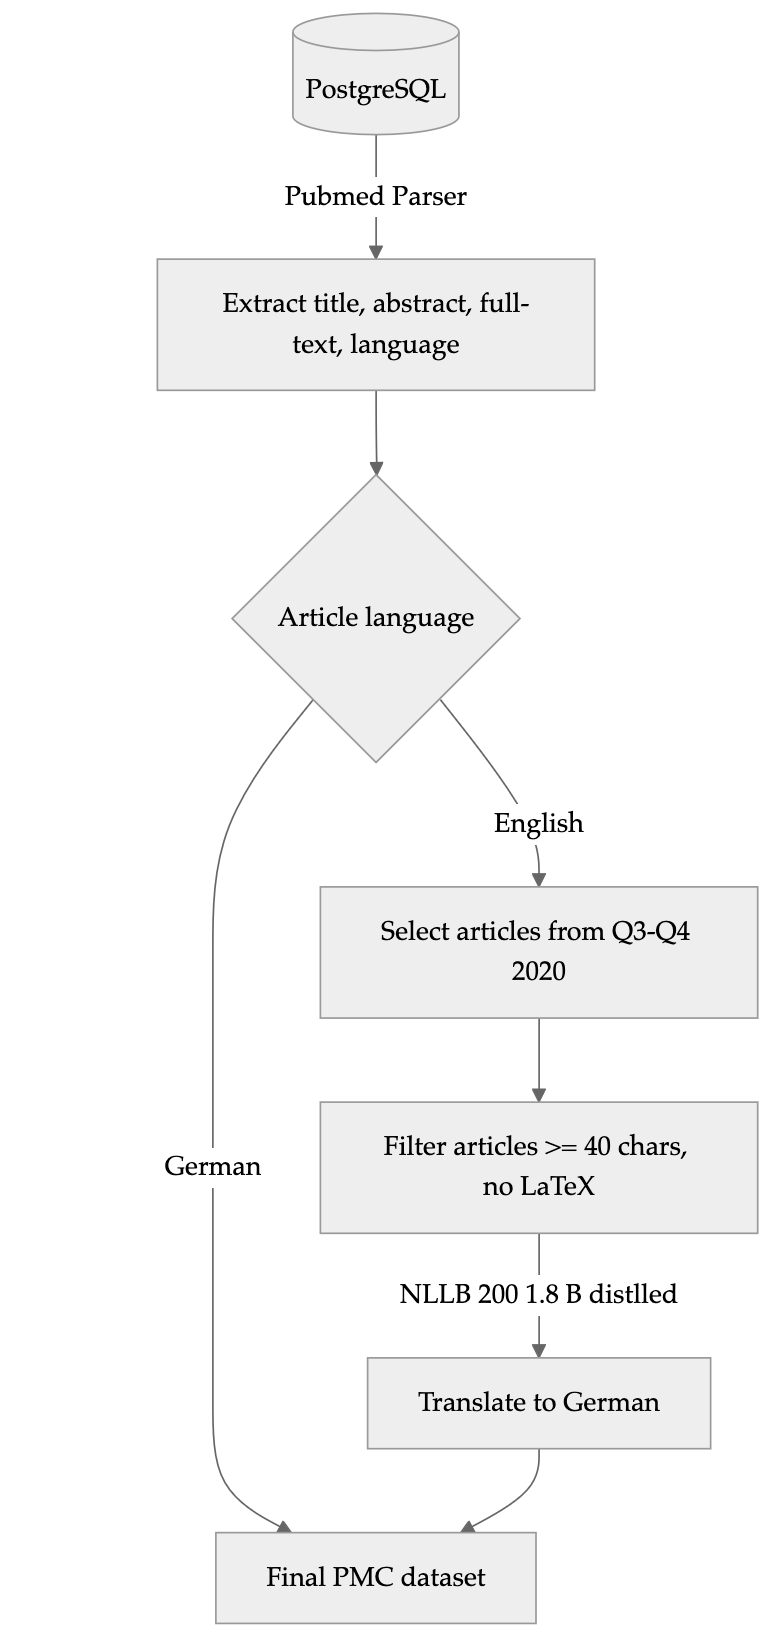
\includegraphics[width=0.5\textwidth]{translation}
    \caption[Flowchart of the PMC translation process]{This flowchart
    illustrates the sequential steps involved in the translation process of
    articles from PubMed Central (PMC). It begins with extracting article
    details from \textsc{PostgreSQL} using \textsc{Pubmed Parser}, followed by
    language-based filtering to select English articles from Q3 and Q4 of 2020.
    Articles are then filtered based on length and \LaTeX{} content, followed by
    translation to German using the NLLB 200 1.3B distilled model.}
    \label{fig:translation}
\end{figure}


\paragraph{PhD Theses} 
In this work, we also included a collection of 7,486 open-access German-language
dissertations and postdoctoral dissertations from Charité University Hospital,
Germany's largest university hospital. At the joint medical faculty of Humboldt
University and Free University of Berlin, electronically published documents,
doctoral and habilitation theses, as well as research data are made available to
the public through the university's institutional repository \textsc{Refubium}
\cite{refubium}. The documents were downloaded in bulk as PDF files and
subsequently converted to plain text. Data cleaning involved removing sentences
that lacked German stop words and excluding theses under 15 pages in length.
This process ensured the inclusion of only relevant, high-quality text data. In
total, 646 MB of text was extracted from the PhD theses.

\paragraph{Medical Wikipedia}
Wikipedia curates entry pages on the encyclopedia about particular subject areas
in so-called \textit{portals}. Each portal acts as a hub, bringing together key
articles, images, and resources about the respective topic. Portals are
particularly useful for getting an organized overview or exploring related
subtopics without searching through individual articles. We utilized the German
Wikipedia portal on medicine in order to extend our pre-training corpus with
freely available texts on medical topics, which were collectively authored and
editorially proofread by a diverse community of volunteer contributors.
Wikipedia does not offer an API for bulk data retrieval, but instead provides an
export interface \cite{wikipediaexport} for downloading specified wiki pages in
a special XML format. These XML files follow a schema specific to
\textsc{MediaWiki}, the software behind Wikipedia, initially intended for
importing into another \textsc{MediaWiki} installation but also allows for
further processing and analysis.

The export interface expects either a list of page titles or a category name,
which it resolves into a list of pages related to the given category. Since our
objective is to crawl the entirety of the medical portal, we implemented a
breadth-first search algorithm on Wikipedia's export interface, employing
\textsc{Selenium WebDriver}~\cite{gojare2015analysis} to traverse the category
tree of the portal. The algorithm starts at the root category
\texttt{Portal:Medizin} and recursively visits each subcategory, collecting the
titles of all pages contained within. The page titles are then used to download
the corresponding XML files in bulk, creating a dump of the entire German
medical portal. The \textsc{MediaWiki} XML files are then converted to plain
text utilizing \textsc{XQuery}, a querying language for finding and extracting
elements and attributes from XML documents. The German Wikipedia portal on
medicine contributes a total of 75,585 documents and 362 MB of data to the
pre-training corpus.

\paragraph{MIMIC-IV Notes}
Medical Information Mart for Intensive Care IV (MIMIC-IV)
\cite{johnson2023mimic} is a large and freely accessible electronic health
record dataset comprising various health-related data acquired during routine
clinical care of patients admitted to critical care units of the Beth Israel
Deaconess Medical Center in Boston, MA, USA. MIMIC-IV constitutes the fourth
edition of the dataset, containing data of over a decade from 2008 to 2019 and
covering a wide range of information such as patient measurements, orders,
diagnoses, procedures, treatments, and clinical notes. 

\begin{table}[htb]
    \centering
    \begin{tabular}{p{0.9\textwidth}}
        \toprule
        \textbf{System Prompt:} \\
        You are an API-like assistant, and output only the plain response
        without further explain or comment the output. \\
        \midrule
        \textbf{User Instruction:} \\
        Translate the following text strictly into German. Do not replace the
        \_\_\_ pseudonymization masks. \texttt{<English Text>} \\
        \bottomrule
    \end{tabular}
    \caption{LLaMA 3.1 system prompt and user instruction used for MIMIC-IV
    translation}
    \label{tab:llama}
\end{table}

For our corpus, we specifically chose to utilize the \textit{clinical notes}
\cite{johnson2023mimicnote} subset of the MIMIC-IV database as it is made up of
discharge summaries written in the form of free text, which is well suited for
training contextual language models. The 330,485 discharge summaries from
145,915 hospitalized patients are organized into sections including chief
complaint, history of present illness, past medical history, brief hospital
course, physical exams, and discharge diagnoses. These free-text notes were
acquired from the hospital system and de-identified by the authors using a
combined automatic approach of custom rules and a neural network trained on
de-identification, cast as a NER task. 

The note subset of the MIMIC-IV dataset is available on \textit{PhysioNet}
\cite{goldberger2000physiobank}, a repository for freely accessible medical data
and tools for computational medicine research. After downloading the collection
of clinical notes, we utilized LLMs to translate the English discharge summaries
to German. Specifically, we employed the multilingual \textit{LLaMA 3.1 8B}
\cite{dubey2024llama3} model in an API-like manner by providing the prompt as
shown in Tab.~\ref{tab:llama}. The translated notes were then included in the
pre-training corpus, consisting of 330,485 documents and 5,310 MB of data.

\paragraph{Web Crawl}
To enrich our corpus with current medical content from the German web, a web
crawl was performed using the implementation described in
\cite{deng2025crawler}, which extends the open-source crawler \textsc{Apache
Nutch}~\cite{khare2004nutch}. The crawl was seeded with a combination of domains
from the \textit{tala-med}~\cite{specht2025evaluating} search engine index as
well as the seed sources provided by the \textit{sampled German Health Web}
(sGHW)~\cite{zowalla2020crawling} project. Tala-med is a search engine providing
high-quality, evidence-based health information, which in its current version
relies on 26 trustworthy German health websites while maintaining strict user
privacy. The sGHW project represents previous efforts to index health-related
web content in the German language and employed a specialized focused crawler to
create an index of 22,405 German health websites. The sGHW index was limited to
websites with \texttt{.de}, \texttt{.at}, and \texttt{.ch} top-level domains,
and used a support vector machine to filter content for health relevance
automatically. Our crawl was configured with parameters \texttt{depth=3} and
\texttt{topN=100}. In web crawling, \texttt{depth} refers to the number of hops
or iterations the crawler will follow links from the seed URL, while the width,
called \texttt{topN}, specifies the maximum number of URLs to fetch in each
iteration. These parameters control the crawling process and were chosen to
allow for systematic exploration of linked content while maintaining a
manageable scope. 

Despite the focused seed list, unsuitable as well as nonmedical content, such as
advertisements, remained present in the crawl data due to the nature of web
crawling. To address this issue, we developed a text classifier in order to
filter medical and scientific content from general web content, ensuring the
relevance of the gathered data. The classifier was built by fine-tuning
GeistBERT on a binary-labeled dataset derived from the scientific portion of the
\textit{10kGNAD}~\cite{10kGNAD} corpus. The 10kGNAD dataset is a subset of the
\textit{One Million Posts Corpus} \cite{schabus2017one} and consists of 10,000
German news articles, including 573 focused on scientific topics. These
scientific articles make up the first half of the fine-tuning dataset, while the
second half was created using a stratified sample to ensure a balanced dataset
and that each category was proportionally represented. The classifier's
performance was evaluated using a manually labeled subset of the web crawl data
of size 119, which was annotated using \textsc{Label Studio}~\cite{labelstudio},
an open-source data labeling tool. On this test set, the classifier achieved an
\ff{} score of 80.34\%, indicating a reliable level of accuracy. Following this
validation, we applied the classifier to filter the complete web crawl dataset.
After filtering, we removed documents from the web crawl with less than 40
characters, those containing the Unicode replacement character \texttt{U+FFFD}
due to encoding issues, and duplicates. For the remaining documents, we removed
phone numbers, email addresses, URLs and emojis utilizing the
\textsc{clean-text} \cite{clean-text} Python library. The preprocessing of the
web crawl resulted in a final collection of 93,642 documents and 512 MB of data.
